\documentclass[11pt]{article}
\usepackage{graphicx}
\usepackage{hyperref}
\usepackage[utf8]{inputenc}
\usepackage{amsmath,amsthm,amsfonts,amssymb,amscd}
\usepackage{tikz}
\usepackage{xeCJK}
\usepackage{physics}
\usepackage{multirow,booktabs}
% \usepackage[table]{xcolor}
\usepackage{fullpage}
\usepackage{lastpage}
\usepackage{unicode-math}
\usepackage{enumitem}
\usepackage{fancyhdr}
\usepackage{mathrsfs}
\usepackage{wrapfig}
\usepackage{setspace}
\usepackage{calc}
\usepackage{multicol}
\usepackage{cancel}
\usepackage[retainorgcmds]{IEEEtrantools}
\usepackage[margin=3cm]{geometry}
\usepackage{amsmath}
\newlength{\tabcont}
\setlength{\parindent}{0.0in}
\setlength{\parskip}{0.05in}
\usepackage{empheq}
\usepackage{framed}
\usepackage[most]{tcolorbox}
\usepackage{xcolor}
\linespread{1.2}
\graphicspath{{./}}
\setCJKmainfont[AutoFakeBold = 3, AutoFakeSlant = 4]{BiauKaiTC}
\colorlet{shadecolor}{orange!15}
\parindent 0in
\parskip 12pt
\geometry{margin=1in, headsep=0.25in}
\graphicspath{{./}}
\theoremstyle{definition}
\newtheorem{thr}{Theorem}
\newtheorem{defn}{Definition}
\newtheorem{reg}{Rule}
\newtheorem{exer}{Exercise}
\newtheorem{note}{Note}
\newtheorem{asmp}{Assumption}
\begin{document}
\setcounter{section}{0}
\title{Title}

\thispagestyle{empty}
\begin{center}
  {\large \bf HTML HW2} \\ 
  B12901022 廖冠豪
\end{center}
\section*{5}
As the boss of the agent, I disagree with its answer and am greatly disappointed by it. The agent claim that it an first fit the polynomial with the $n - 1$. However $n - 1$ equations isn't enough to specify the $n + 1$ coefficients in the $n$-degree polynomial. Next the agent say that with the polynomial, the $n + 1$-th term of the sequence can be determined This step is correct. The agent then provides an example. In the example, the agent fits the polynomial of degree $2$ with three points. The example is correct because $3$ equations is sufficient for specifying a second degree polynomial. In conclusion, the agent displayed poor mathematical ability by giving positive reply to a mathematically impossible task. It further shows bad logical consistency by trying to prove its false statement with an example that is correct itself but has no significance with respect to the statement.
\newpage
\section*{6}
% We divide the number into four groups
% \begin{gather*}
%   W = {1, 3, 5, 7} \\ 
%   X = {2, 4, 6, 8} \\ 
%   Y = {9, 11, 13, 15} \\ 
%   Z = {10, 12, 14, 16} \\
% \end{gather*}
% We denote the number drawn 
Notice that given any number, the color of it when it is on a A ticket is different to it's color when it is on a B ticket. Similarly, it's color when it is on a C ticket is different to it's color when it is on a D ticket. Therefore, some number on the five tickets to be purely green, that five tickets can't contain A and C tickets at the same time, or B and D tickets at the same time. \\ 
When all the tickets are A or C, all the numbers $9, 11, 13, 15$ are green, and the condition is satisfied. When all the tickets are B or D, all the numbers $2, 4, 6, 8$ are green. When all the tickets are A or D, all the numbers $1, 3, 5, 7$ are green. When all the numbers are B or C, all the numbers $10, 12, 14, 16$ are green. The condition is also satisfied when all the tickets are of the same alphabet.
% From the analysis above, we know that the probability that the condition is met is the probability that all the tickets are A or C plus the probability that all the tickets are B or D. 
Also, since that number of the four kinds of tickets are of the same large quantity, the probability for each drawn ticket to have any specific alphabet is $\frac{1}{4}$.
\begin{gather*}
  P = \underset{AC, AD, BC, BD}{4}\times(\underset{}{(\frac{1}{2})^5} -  2\times\underset{}{(\frac{1}{4})^5}) + \underset{A, B, C, D}{4}\times(\frac{1}{4})^5 \\ 
  = \frac{31}{256}
\end{gather*}
\newpage
\section*{7}
In order that the 5 on a ticket is green, this ticket must be of alphabet A or D. 
\[
  P = (\underset{A}{\frac{1}{4}} + \underset{D}{\frac{1}{4}})^5 = \frac{1}{32}
\]
\newpage
\section*{8}
% \sum_{t^\prime = M + 1}^\infty
We first consider the probability for all $m$ at a fixed $t = t^\prime$.
\begin{gather*}
  P\left(\forall m\in \{1, 2,\dots, M\}\quad \mu_m\leq\frac{c_m}{N_m}+\sqrt{\frac{\ln{t^\prime}+\ln{M} -\frac{1}{2}\ln{\delta}}{N_m}} | t = t^\prime\right) \\ 
  = 1 - P\left((\mu_1 > \frac{c_1}{N_1} + \sqrt{\frac{\ln{t^\prime} + \ln{M} -\frac{1}{2}\ln{\delta}}{N_1}})\cap\dots\cap(\mu_M > \frac{c_M}{N_M} + \sqrt{\frac{\ln{t^\prime} + \ln{M} -\frac{1}{2}\ln{\delta}}{N_M}}) | t = t^\prime\right) \\
  \geq 1 - \sum_{m\in{1, 2,\dots,M}}P\left(\mu_m < \frac{c_m}{N_m} + \sqrt{\frac{\ln{t^\prime} - \frac{1}{2}\ln{\frac{\delta}{M^2}}}{N_m}}\right)
\end{gather*}
Since $0 < \frac{\delta}{M^2} < 1$, we can use the inequality provided in this problem.
\begin{gather*}
  \geq 1 - \sum_{m\in{1, 2,\dots,M}}\frac{\delta}{M^2}t^{-2} = \frac{\delta}{M}t^{-2}
\end{gather*}
Let $A$ denote the event $\forall m \in {1, 2,\dots, M}\quad \mu_m > \frac{c_m}{N_m} + \sqrt{\frac{\ln{t^\prime} + \ln{M} -\frac{1}{2}\ln{\delta}}{N_m}}$, our result in the previous part show that
\begin{gather*}
  P(A | t = t^\prime) \geq 1 - \frac{\delta}{M}t^{-2} \\ 
  \implies P(A^\prime | t = t^\prime) \leq \frac{\delta}{M}t^{-2}
\end{gather*}
\begin{gather*}
  P\left(\forall m\in \{1, 2,\dots, M\}, t \in \{M + 1, M + 2,\dots\} \quad\mu_m\leq\frac{c_m}{N_m}+\sqrt{\frac{\ln{t^\prime}+\ln{M} -\frac{1}{2}\ln{\delta}}{N_m}} \right) \\ 
  = P((A | t = M + 1) \cap (A | t = M + 2) \cap\dots) \\ 
  = 1 - P((A^\prime | t = M + 1) \cap (A^\prime | t = M + 2) \cap\dots) \\
  \geq 1 - \sum_{t^\prime = m + 1}^\infty P(A^\prime | t = t^\prime) \\ 
  \geq 1 - \sum_{t^\prime = m + 1}^\infty \frac{\delta}{M}{t^\prime}^{-2}
  \geq 1 - \frac{\delta}{M} \sum_{t^\prime = 1}^\infty {t^\prime}^{-2} \\ 
  = 1 - \frac{\pi^2\delta}{6M} \\
  \geq 1 - \delta \quad(\frac{\pi^2}{6M} < 1 \quad\text{for}\quad M \geq 2) \\
\end{gather*}
\newpage
\section*{9}
\textbf{The VC bound of the set of symmetric boolean functions is k + 1} \\ 
Proof: \\
First we prove that $d_{VC} \leq k + 1$ \\ 
When there is more than $k + 1$ vectors $\vb{v}\in \{-1, 1\}^k$, pigeonhole principal states that there must exist two vectors $\vb{v}_1, \vb{v}_2$ that has the same number of ones. Since the functions are symmetric, the output they produce given $\vb{v}_1$ and $\vb{v}_2$ must be the same. Therefore, any data set with more than $k + 1$ vectors can't be scattered, and $d_{VC} \leq k + 1$ \\
Next we prove that $d_{VC} \geq k + 1$ \\ 
Consider a data set with $n \geq k + 1$ vectors such that no two vectors have the same number of ones. For any dichotomy, we divide the vectors into two groups, one containing all the vectors with $+1$ as their output, and the other with all the vectors with $-1$. 
  Let $h: \{-1, +1\}^k \rightarrow\{-1, +1\}$ be the boolean function such that for all vectors $\vb{v}$ in this data set $h(\vb{v})$ is equal to its output. Since no two vectors in different groups have the same number of ones, $h$ is symmetric and hence belong to our hypothesis set. Hence the $n$ vectors can be scattered, and $d_{VC} \geq k + 1$. \\ 
  Since $d_{VC} \leq k + 1$ and $d_{VC} \geq k + 1$, we've proven that $d_{VC} = k + 1$.
\newpage
\section*{10}
\begin{gather*}\\
  E_{out} = P[h(x) = +1\cap y = -1] + P[h(x) = -1\cap y = +1] \\ 
  = P[s(x - \theta) > 0 \cap x > 0 \cap y = -1]\\ +  P[s(x - \theta) > 0 \cap x \leq 0 \cap y = -1] \\+  P[s(x - \theta) \leq 0 \cap x > 0 \cap y = +1] \\ +  P[s(x - \theta) \leq 0 \cap x \leq 0 \cap y = +1]
\end{gather*}
We classify the problem into four cases and treat them separately. \\ 
\subsection*{}
$s = +1, \theta\geq0$\\
\begin{gather*}
  E_{out} = \frac{1 - \theta}{2}p + 0 + \frac{\theta}{2}(1 - p) + \frac{p}{2} \\ 
  = p + \frac{\theta}{2} - p\theta
\end{gather*}
\subsection*{}
$s = +1, \theta < 0$ \\ 
\begin{gather*}
  E_{out} = \frac{p}{2} + \frac{-\theta}{2}(1 - p) + 0 + \frac{\theta + 1}{2}p \\ 
  = p - \frac{\theta}{2} + p\theta
\end{gather*}
\subsection*{}
$s = -1, \theta\geq0$\\
\begin{gather*}
  E_{out} = \frac{\theta}{2}p + \frac{1}{2}(1 - p) + \frac{1 - \theta}{2}(1 - p) + 0 \\ 
  = 1 - p + p\theta - \frac{\theta}{2}
\end{gather*}
$s = -1, \theta<0$\\
\begin{gather*}
  E_{out} = 0 + \frac{\theta + 1}{2}(1 - p) + \frac{1}{2}(1 - p) + \frac{-\theta}{2}p \\ 
  = 1 + \frac{\theta}{2} - p\theta - p
\end{gather*}
By the analysis above, we can conclude that for any $h_{s, \theta}$ with $s \in {-1, +1}$ and $\theta \in [-1, 1]$, 
\[
  E_{out}(h_{s, \theta}) = u + v\cdot\abs{\theta}
\]
With 
\begin{gather*}
  u = s(\frac{1}{2} - p) \\ 
  v = \frac{1}{2} - u
\end{gather*}
\newpage
\section*{11}
Scatter plot: \\ 
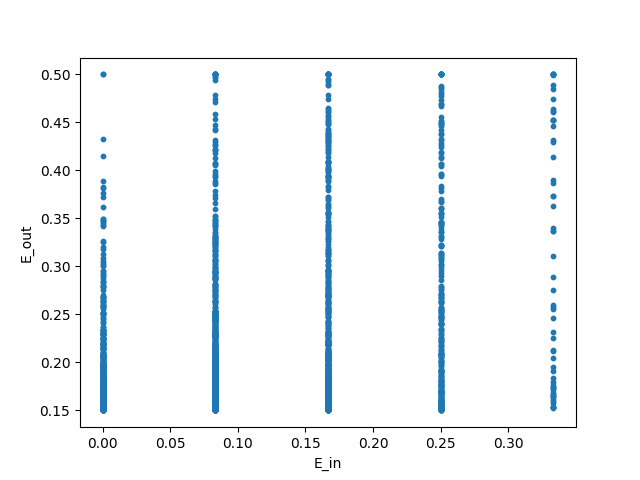
\includegraphics{P11_2.png} \\
\textbf{Median: 1.271091} \\
We see from the scatter plot that all the hypotheses has $E_{out} = 0, 0.08333, 0.166667, 0.25, 0.333333$, which correspond to $0, 1, 2, 3, 4$ errors in the $12$ data points respectively. This means that in the learning processes, no hypothesis that makes more than $4$ error are returned. This is reasonable because the learning algorithm returns the hypothesis with minimal $E_{in}$. \\ 
Code Snapshot: \\ 

\includegraphics[width = \textwidth]{P11code.png}
\newpage
\section*{12}
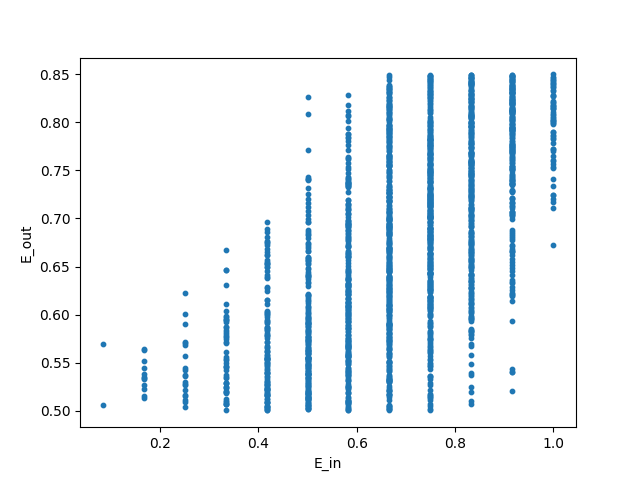
\includegraphics{P12_2.png} \\
\textbf{Median: -0.029372} \\
We see from the scatter plot that in contrast to P11, the number of errors range from $0$ to $12$, this is also reasonable because in this cases we return a random hypothesis instead of an optimal one. We can also see that for larger $E_{out}$ values, the probability for their corresponding $E_{in}$ to be larger is higher. This means that there is a positive relation between $E_{out}$ and $E_{in}$. This is as expected, since Hoeffding's inequality state that the probability of a large difference between $E_{out}$ and $E_{in}$ is upper-bounded. That is to say, $E_{out}$ is close to $E_{in}$ with a considerable probability. \\
Also, we see that the median of $E_{out} - E_{in}$ in P12 is significantly smaller than that in P11. Observe that for hypotheses with a higher number of errors, $E_{in}$ is higher than $E_{out}$ (as can be seen in the case where 12 errors are made and $E_{in}$ is 1 while $E_{out}$ is less than 1), and for hypotheses with a lower number of errors, $E_{in}$ is lower than $E_{in}$ (as can be seen in the case where 0 error is made and $E_{in}$ is 0 while $E_{out}$ is greater than 0). This explains why in P11, where hypotheses with lower $E_{in}$ are chosen, the median of $E_{in} - E_{out}$ is greater than that in P12, where hypotheses are randomly (and uniformly) chosen.  \\
Code Snapshot: \\ 

\includegraphics[width =\textwidth]{P12code.png}
% \newpage
% \section*{13}
% \textbf{This problem is done in collaboration with B12901035 鄭宇彥}
% Let $\mathcal{H}_{i^\prime}$ be the subset of $\mathcal{H}$ that contains all hypotheses $h_{s, i, \theta}$ of one specific dimension $i = i^\prime$. Clearly this set of hypotheses can only produce $2n$ dichotomies, as the 1D case of this problem is simply the positive ray. Therefore, with $2^n$ dichotomies and $d$ dimensions in total we achieve a bound for $n$ such that the data vectors can be scattered.
% \[
%   2nd \geq 2^n
% \]
% We then apply this bound to $d_{VC}$ \\ 
% \begin{align*}
%   2d_{VC}d \geq 2^{d_{VC}} \\ 
%   \implies d_{VC} &\leq \lg(2d_{VC}d) = 1 + \lg{d} + \lg{d_{VC}}  \\
%   &\leq 1 + \lg{d} + \lg(1 + \lg{d} + \lg{d_{VC}})
% \end{align*}
\end{document}
